% Preamble
\documentclass[a4paper,12pt]{article}

\usepackage[osf]{mathpazo} % palatino
%\usepackage{ms1}            % load the template
%\usepackage[round]{natbib} % author-year citations
\usepackage[superscript,biblabel]{cite} % for superscript citations
\usepackage{graphicx}
\usepackage{subcaption}
\usepackage{parskip} 
\usepackage{amsmath}
\usepackage{textcomp} % for parts per mille symbol  
\usepackage{pdflscape} % landscape   
\pagenumbering{arabic}    
\linespread{1.66}



% -------------------------------------------------------------------------------------------------------
% some custom commands

% Add support for highlighting
\usepackage{color}
\newcommand{\hilight}[1]{\colorbox{yellow}{#1}}

% figure numbering override
\renewcommand*{\thefigure}{S\arabic{figure}} % make Fig S1 not Fig 1
\renewcommand*{\thetable}{S\arabic{table}} % make Table S1 not Table 1

% -------------------------------------------------------------------------------------------------------

% Title page information
\title{Supplementary Information from:\\
\textit{Reconstructing the last known movements of one of Nature's giants}}
% 90 characters max

\author{Clive N. Trueman, Andrew L. Jackson, Katharyn S. Chadwick,\\ 
Ellen J. Coombs, Richard C. Sabin and Natalie Cooper}

\date{}


%\vfill


% End of preamble

\begin{document}
%\title{Supplementary Information - Cooper et al. 2017}
%\modulolinenumbers[1]   % Line numbering on every line

\maketitle

\parindent = 1.5em
\addtolength{\parskip}{.3em}


\section*{Supplementary Methods}
 
\subsection*{CHARACTERISATION OF THE MEASURED BALEEN}
The baleen plate yielded 78 discrete samples of baleen. 
Across the baleen sample, $\delta^{15}$N values show clear cycles with periods of relatively high $\delta^{15}$N values interspersed by relatively short periods where $\delta^{15}$N values are c.1\text{\textperthousand} lower. 
Fourier analysis (periodogram function in the R package TSA\cite{Chan:2012aa}) revealed a strong periodic repetition with a 13.3cm periodicity. 
The oldest 35cm of the baleen plate  record relatively positive and constant $\delta^{13}$C values, associated with a weakening of the periodic fluctuation seen in $\delta^{15}$N values, and an overall reduction in $\delta^{15}$N values. 
$\delta^{13}$C values also show repeated fluctuations in the middle 50cm of the baleen plate (behavioural phase two), with a similar periodicity of 13.5cm (Fig. \ref{figs1}). 
A distinct change in the isotopic pattern along the baleen plate occurs at around 84cm in behavioural phase two, with a transition to uniform, relatively low $\delta^{13}$C values followed by an abrupt transition to positive $\delta^{13}$C values and a decline in $\delta^{13}$C values in the last 3cm of the record.

% figure s1
\begin{figure}[!htbp]
  \centering
  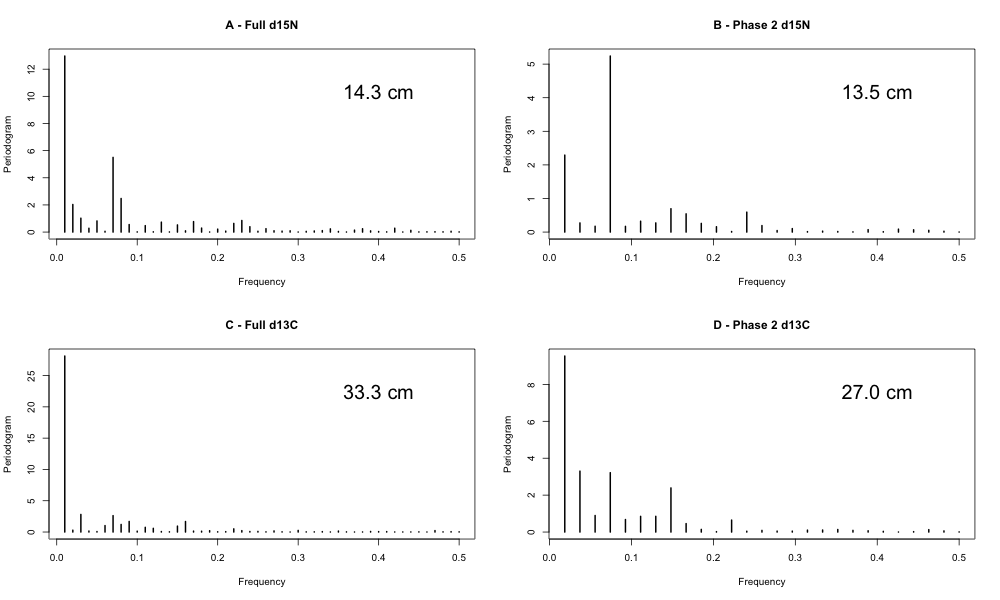
\includegraphics[width = \linewidth]{figures/Figure-S1-periodograms.png}
  \caption{Fourier analysis of $\delta^{15}$N (A,B) and $\delta^{13}$C (C,D) values of the full (A,C) and behavioural phase one only (B,D) components of the baleen plate. Inset values are the highest frequency spectral densities (in cm), excluding the values at the edge of the baleen (i.e. 80cm), and at the sharp increase of $\delta^{13}$C seen at 60cm. Periodic fluctuation with a distance of 13.5cm along the baleen plate is consistently recovered, but is weaker or absent in behavioural phase two.} 
  \label{figs1}
\end{figure}
 
Cross-correlation analysis demonstrates a strong negative covariance between $\delta^{13}$C and $\delta^{15}$N  values within behavioural phase two (Fig. \ref{figs2}), but no relationship between $\delta^{13}$C and $\delta^{15}$N values exists during behavioural phase one.

% figure s2
\begin{figure}[!htbp]
  \centering
  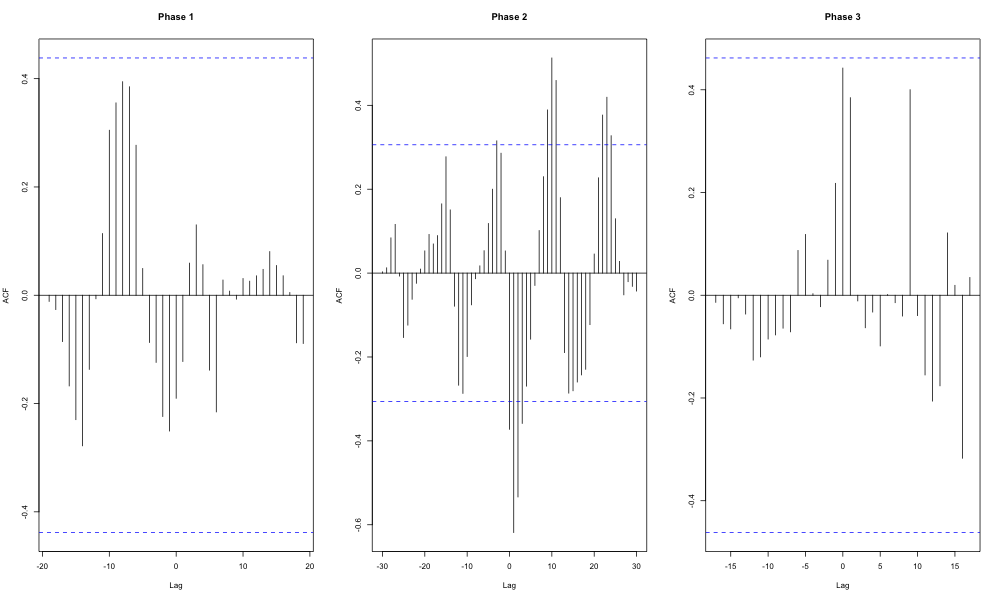
\includegraphics[width = \linewidth]{figures/Figure-S2-cross-cor.png}
  \caption{Cross correlation between $\delta^{13}$C and $\delta^{15}$N values for behavioural phase one showing strong negative covariance with a periodicity of around 13cm.} % check legend
  \label{figs2}
\end{figure}
 
\subsection*{BASELINE ISOTOPE COMPARISONS}
Isotope-enabled biogeochemical ocean models\cite{magozzi2017using,schmittner2016complementary} were used to characterise the isotopic composition of phytoplankton expected in different potential foraging grounds. 
Annual average $\delta^{15}$N POM values were provided by C.J. Somes (pers.comm) based on a 5$^{\circ}$ resolution biogeochemical model. 
$\delta^{13}$C POM values were simulated using an isotopic extension to the NEMO-MEDUSA model\cite{magozzi2017using}.
 
Simulated $\delta^{15}$N POM values are relatively positive in the northeast Atlantic north of c.60$^{\circ}$N, and relatively negative in the central and southern North Atlantic, associated with high levels of nitrogen fixation (Fig. \ref{figs3}). 
Annual average $\delta^{13}$C POM values largely vary with latitude, with more negative values in more northerly regions. 
In the central North Atlantic, $\delta^{13}$C POM values are relatively positive in the west, reflecting warm gulf stream waters (Fig. \ref{figs3}). 
The temporally coincident periodic, inverse fluctuations in $\delta^{13}$C and $\delta^{15}$N values in the initial phase of the baleen plate are therefore consistent with migration between waters north of 60$^{\circ}$N and more southerly southern waters in the North Atlantic, with northerly occupancy in summer months and southerly occupancy in winter months. 
Incorporation of carbon and nitrogen with isotopic ratios consistent with southerly latitudes during winter months indicates continued feeding during migration and winter residency.
 
\begin{figure}[!htbp]
    \centering
    \begin{subfigure}[t]{0.45\textwidth}
        \centering
        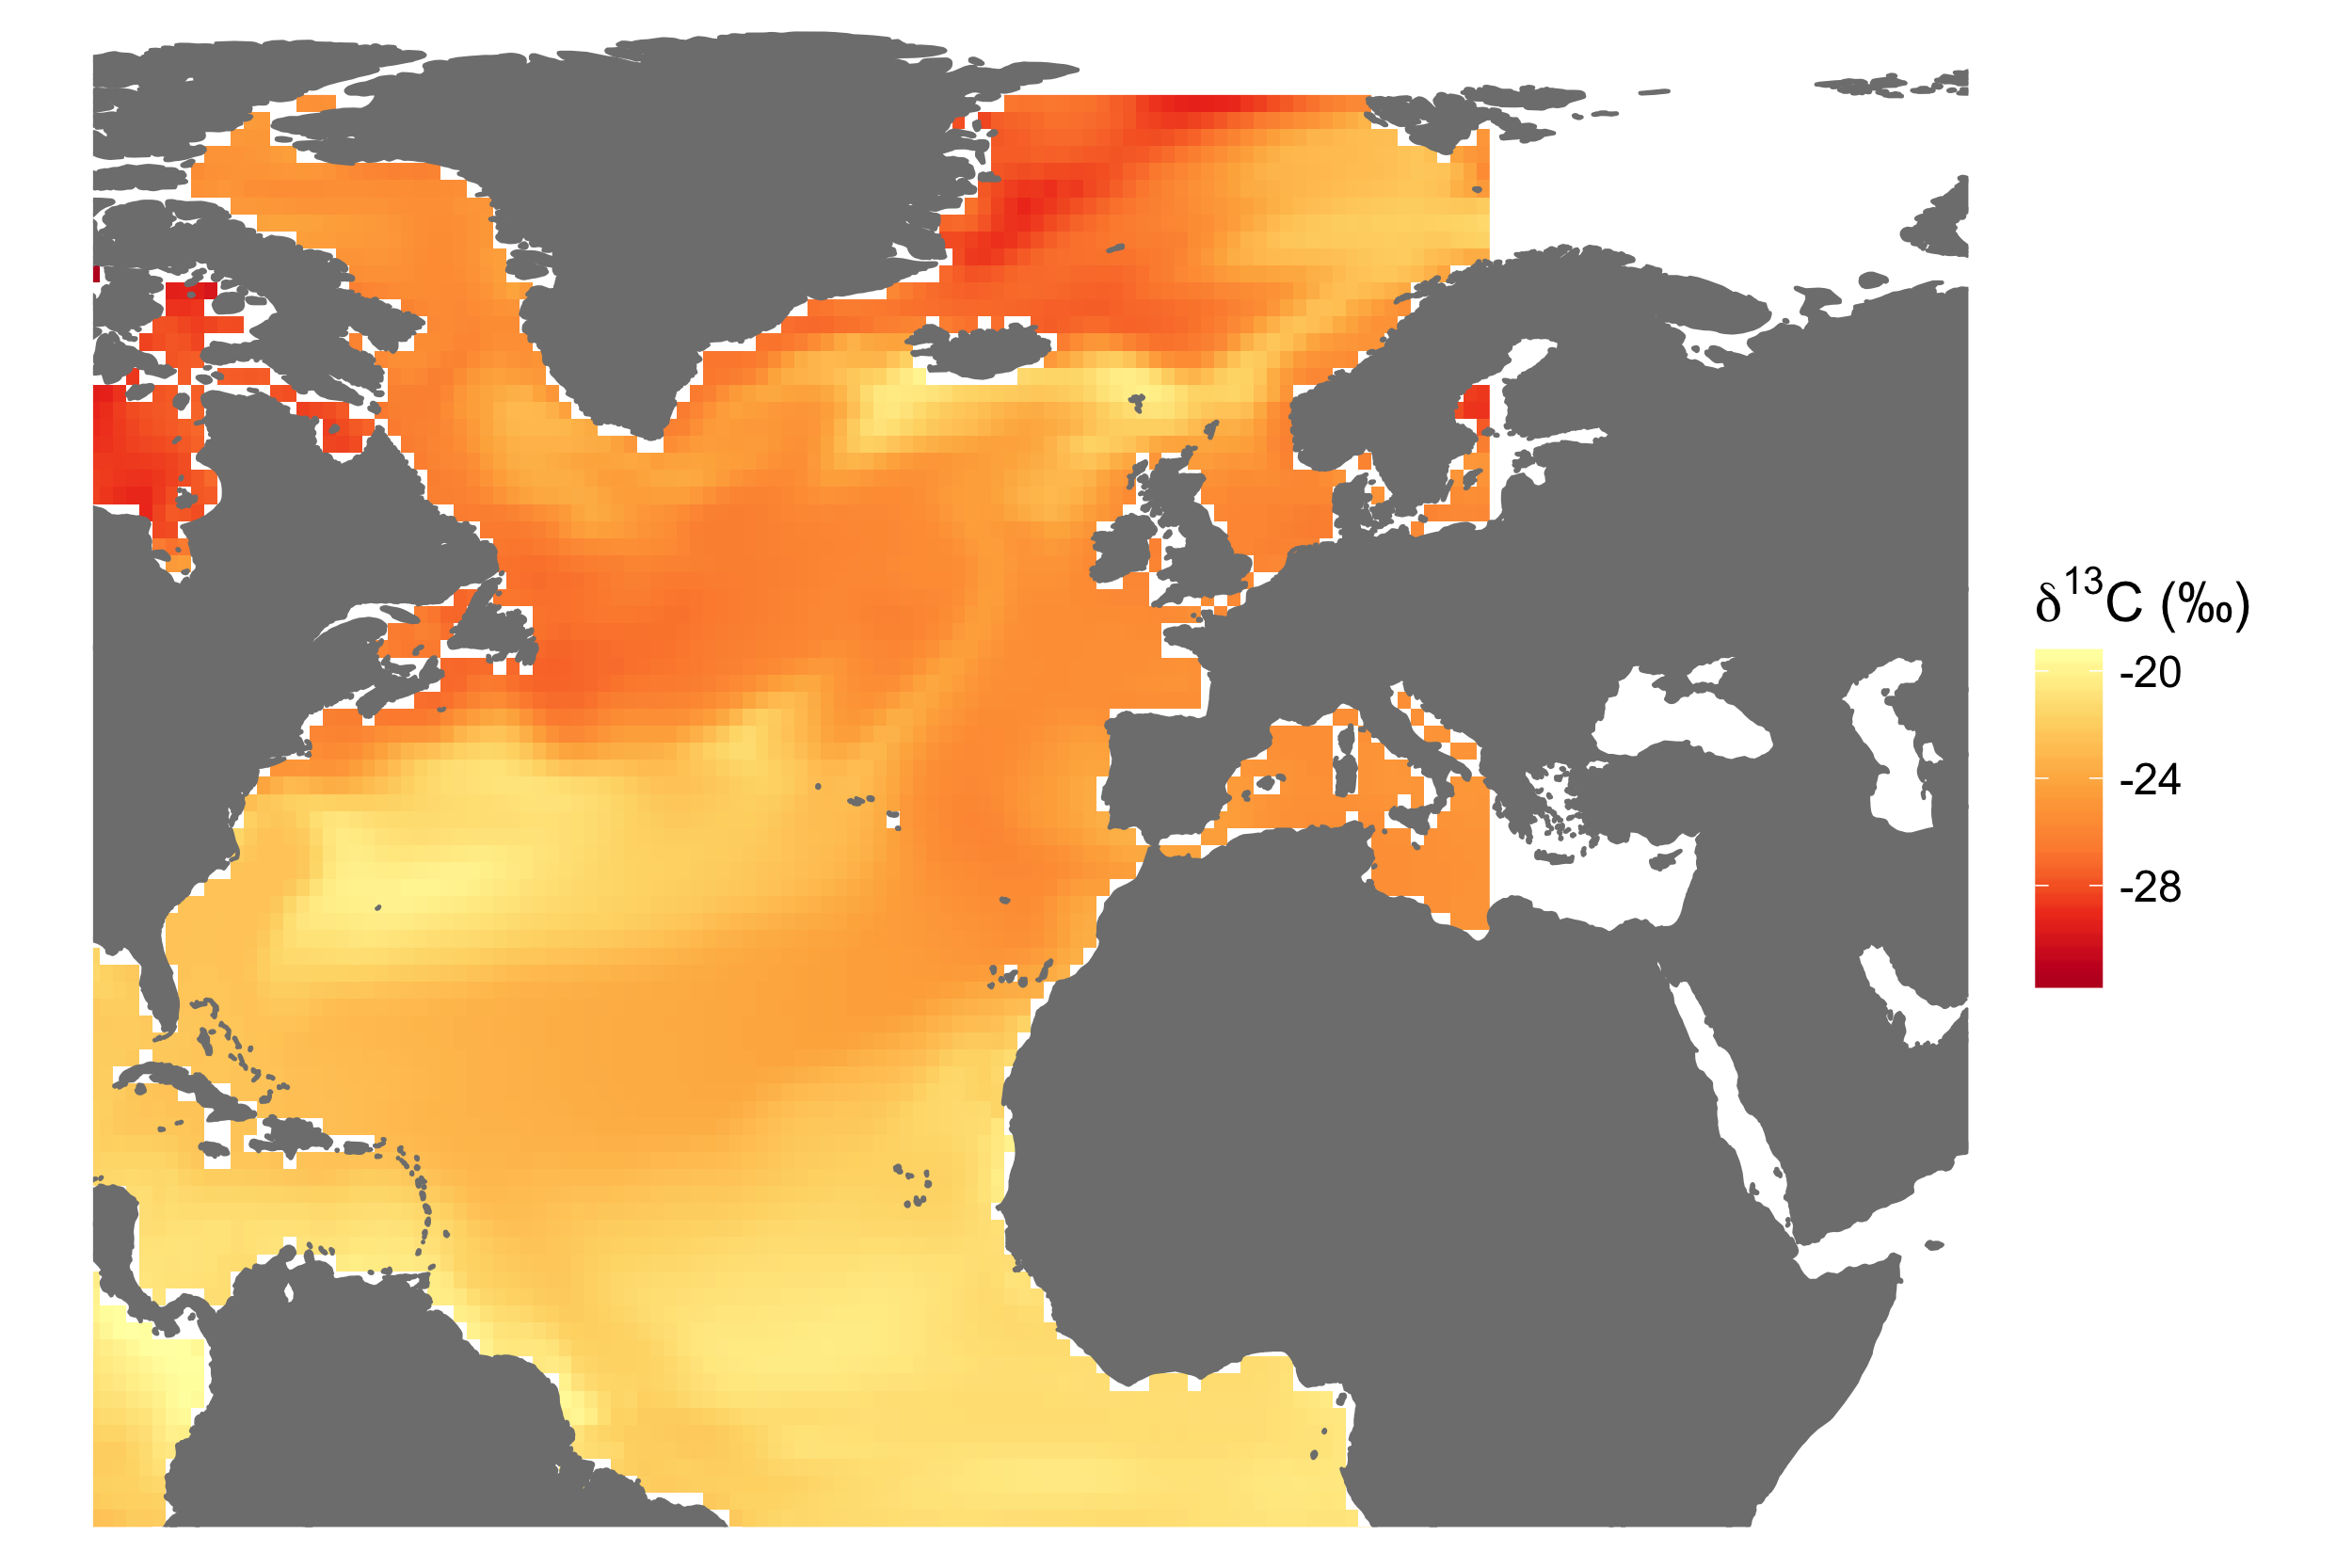
\includegraphics[width=\linewidth]{figures/Figure-S3-plankton-d13C-map.png} 
    \end{subfigure}
    \hfill
    \begin{subfigure}[t]{0.45\textwidth}
        \centering
        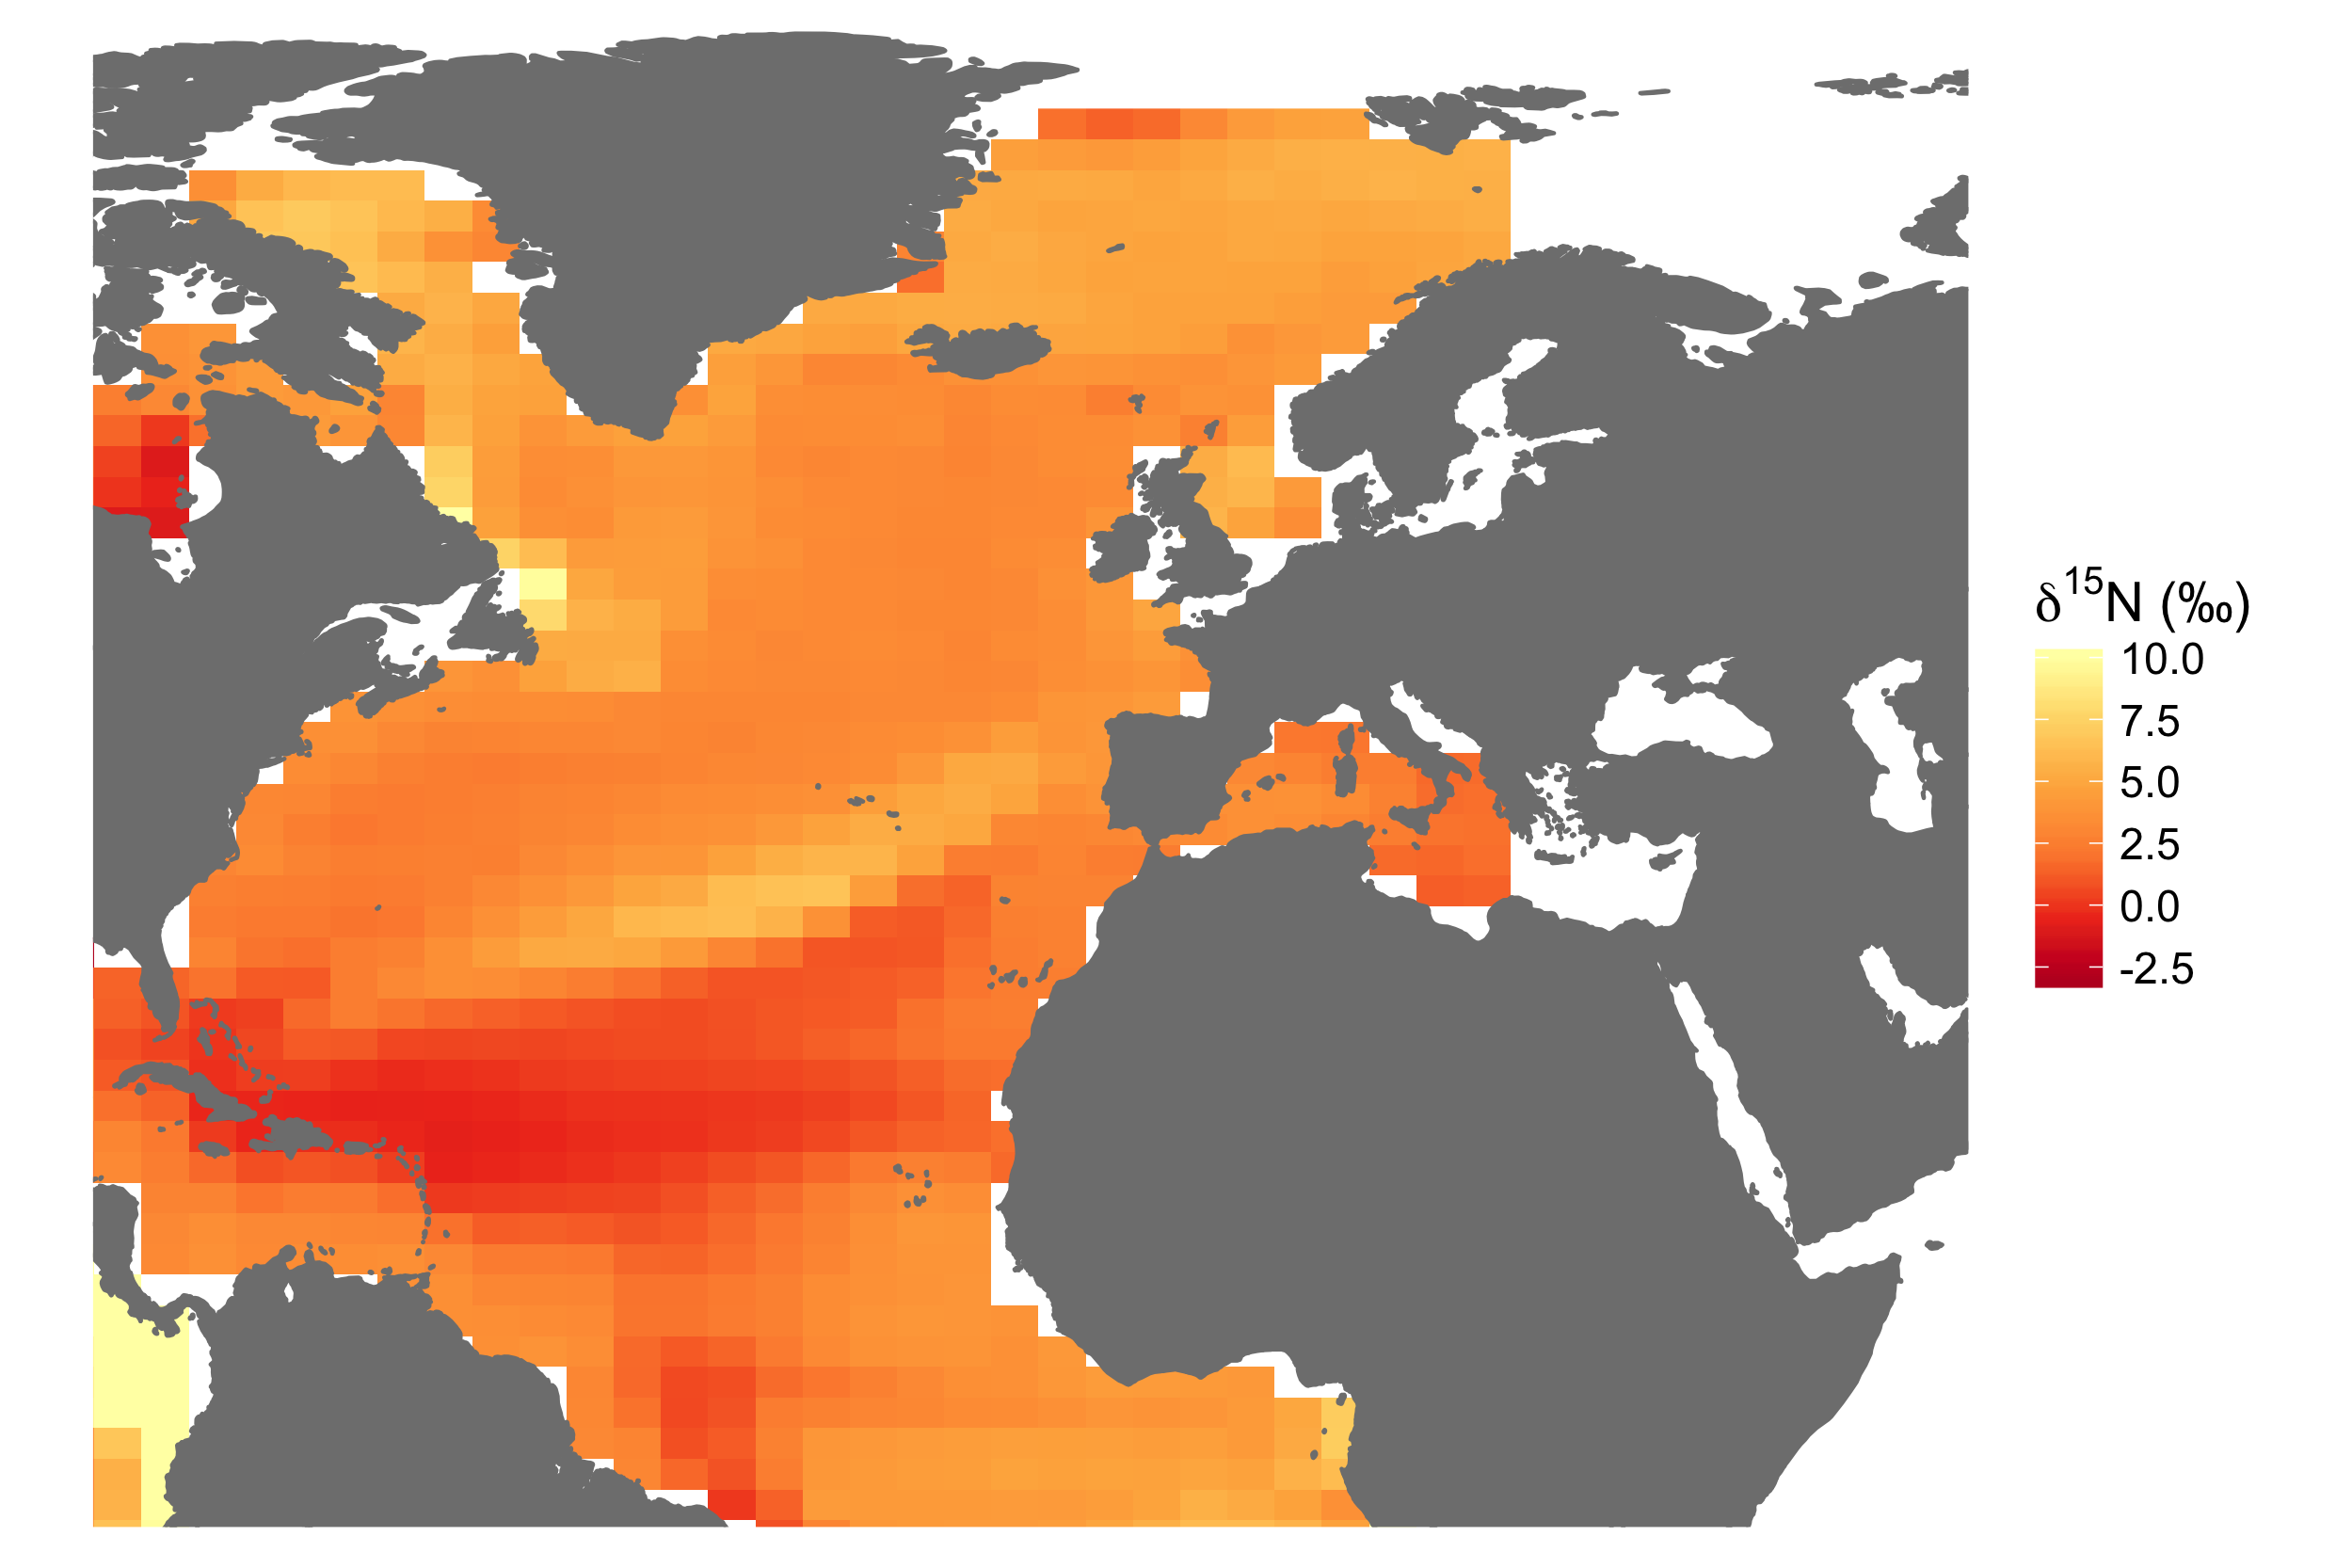
\includegraphics[width=\linewidth]{figures/Figure-S3-plankton-d15N-map.png} 
    \end{subfigure}
    \caption{Spatial model (isoscape) of model-simulated biomass weighted annual average $\delta^{13}$C (left) and $\delta^{15}$N (right) values from POM. $\delta^{13}$C values are from Magozzi et al. 2017\cite{magozzi2017using} and $\delta^{15}$N from Schmittner \& Somes 2016\cite{schmittner2016complementary} and C.J. Somes (pers. comm.).} 
    \label{figs3}
\end{figure}

The isotopic composition of carbon in phytoplankton also varies through seasons as isotopic fractionation of carbon during photosynthesis is strongly influenced by sea surface temperature\cite{laws1995dependence}. 
Thus temporal variations in $\delta^{13}$C POM values are superimposed on latitudinal gradients. 
The scale and nature of temporal variation in $\delta^{13}$C POM values also varies with latitude, with higher latitude seas showing greater intra-annual variation in $\delta^{13}$C POM values linked to strongly seasonal phytoplankton growth dynamics. 
We therefore used monthly simulated $\delta^{13}$C POM values to simulate the isotopic expression of phytoplankton expected to be encountered by whales exhibiting differing movement behaviours.
 
\subsection*{ISOTOPE MODEL SIMULATIONS}
We initially simulated temporal variations in baseline (phytoplankton) isotopic compositions that would be encountered by whales foraging within broad geographic regions (west UK/Irish shelf, Norwegian/Barents Sea, Canaries/west Azores, Mid Atlantic ridge; Fig. \ref{figs4}). 
Strong seasonal dynamics in $\delta^{13}$C values are evident in all northerly regions, characterized by a rapid increase to annual maximum $\delta^{13}$C values associated with the onset of the spring phytoplankton bloom, followed by more gradual decline in $\delta^{13}$C values towards minima in winter conditions (Fig. \ref{figs4}). 
In temperate latitudes around the British Isles, seasonal dynamic cycles are present, but dampened (Fig. \ref{figs4}), whereas in subtropical regions exemplified by the Canaries and western Azores/Mid Atlantic ridge areas, $\delta^{13}$C values are relatively positive and constant throughout the year (Fig. \ref{figs4}).
 
  \begin{figure}[!htbp]
    \centering
      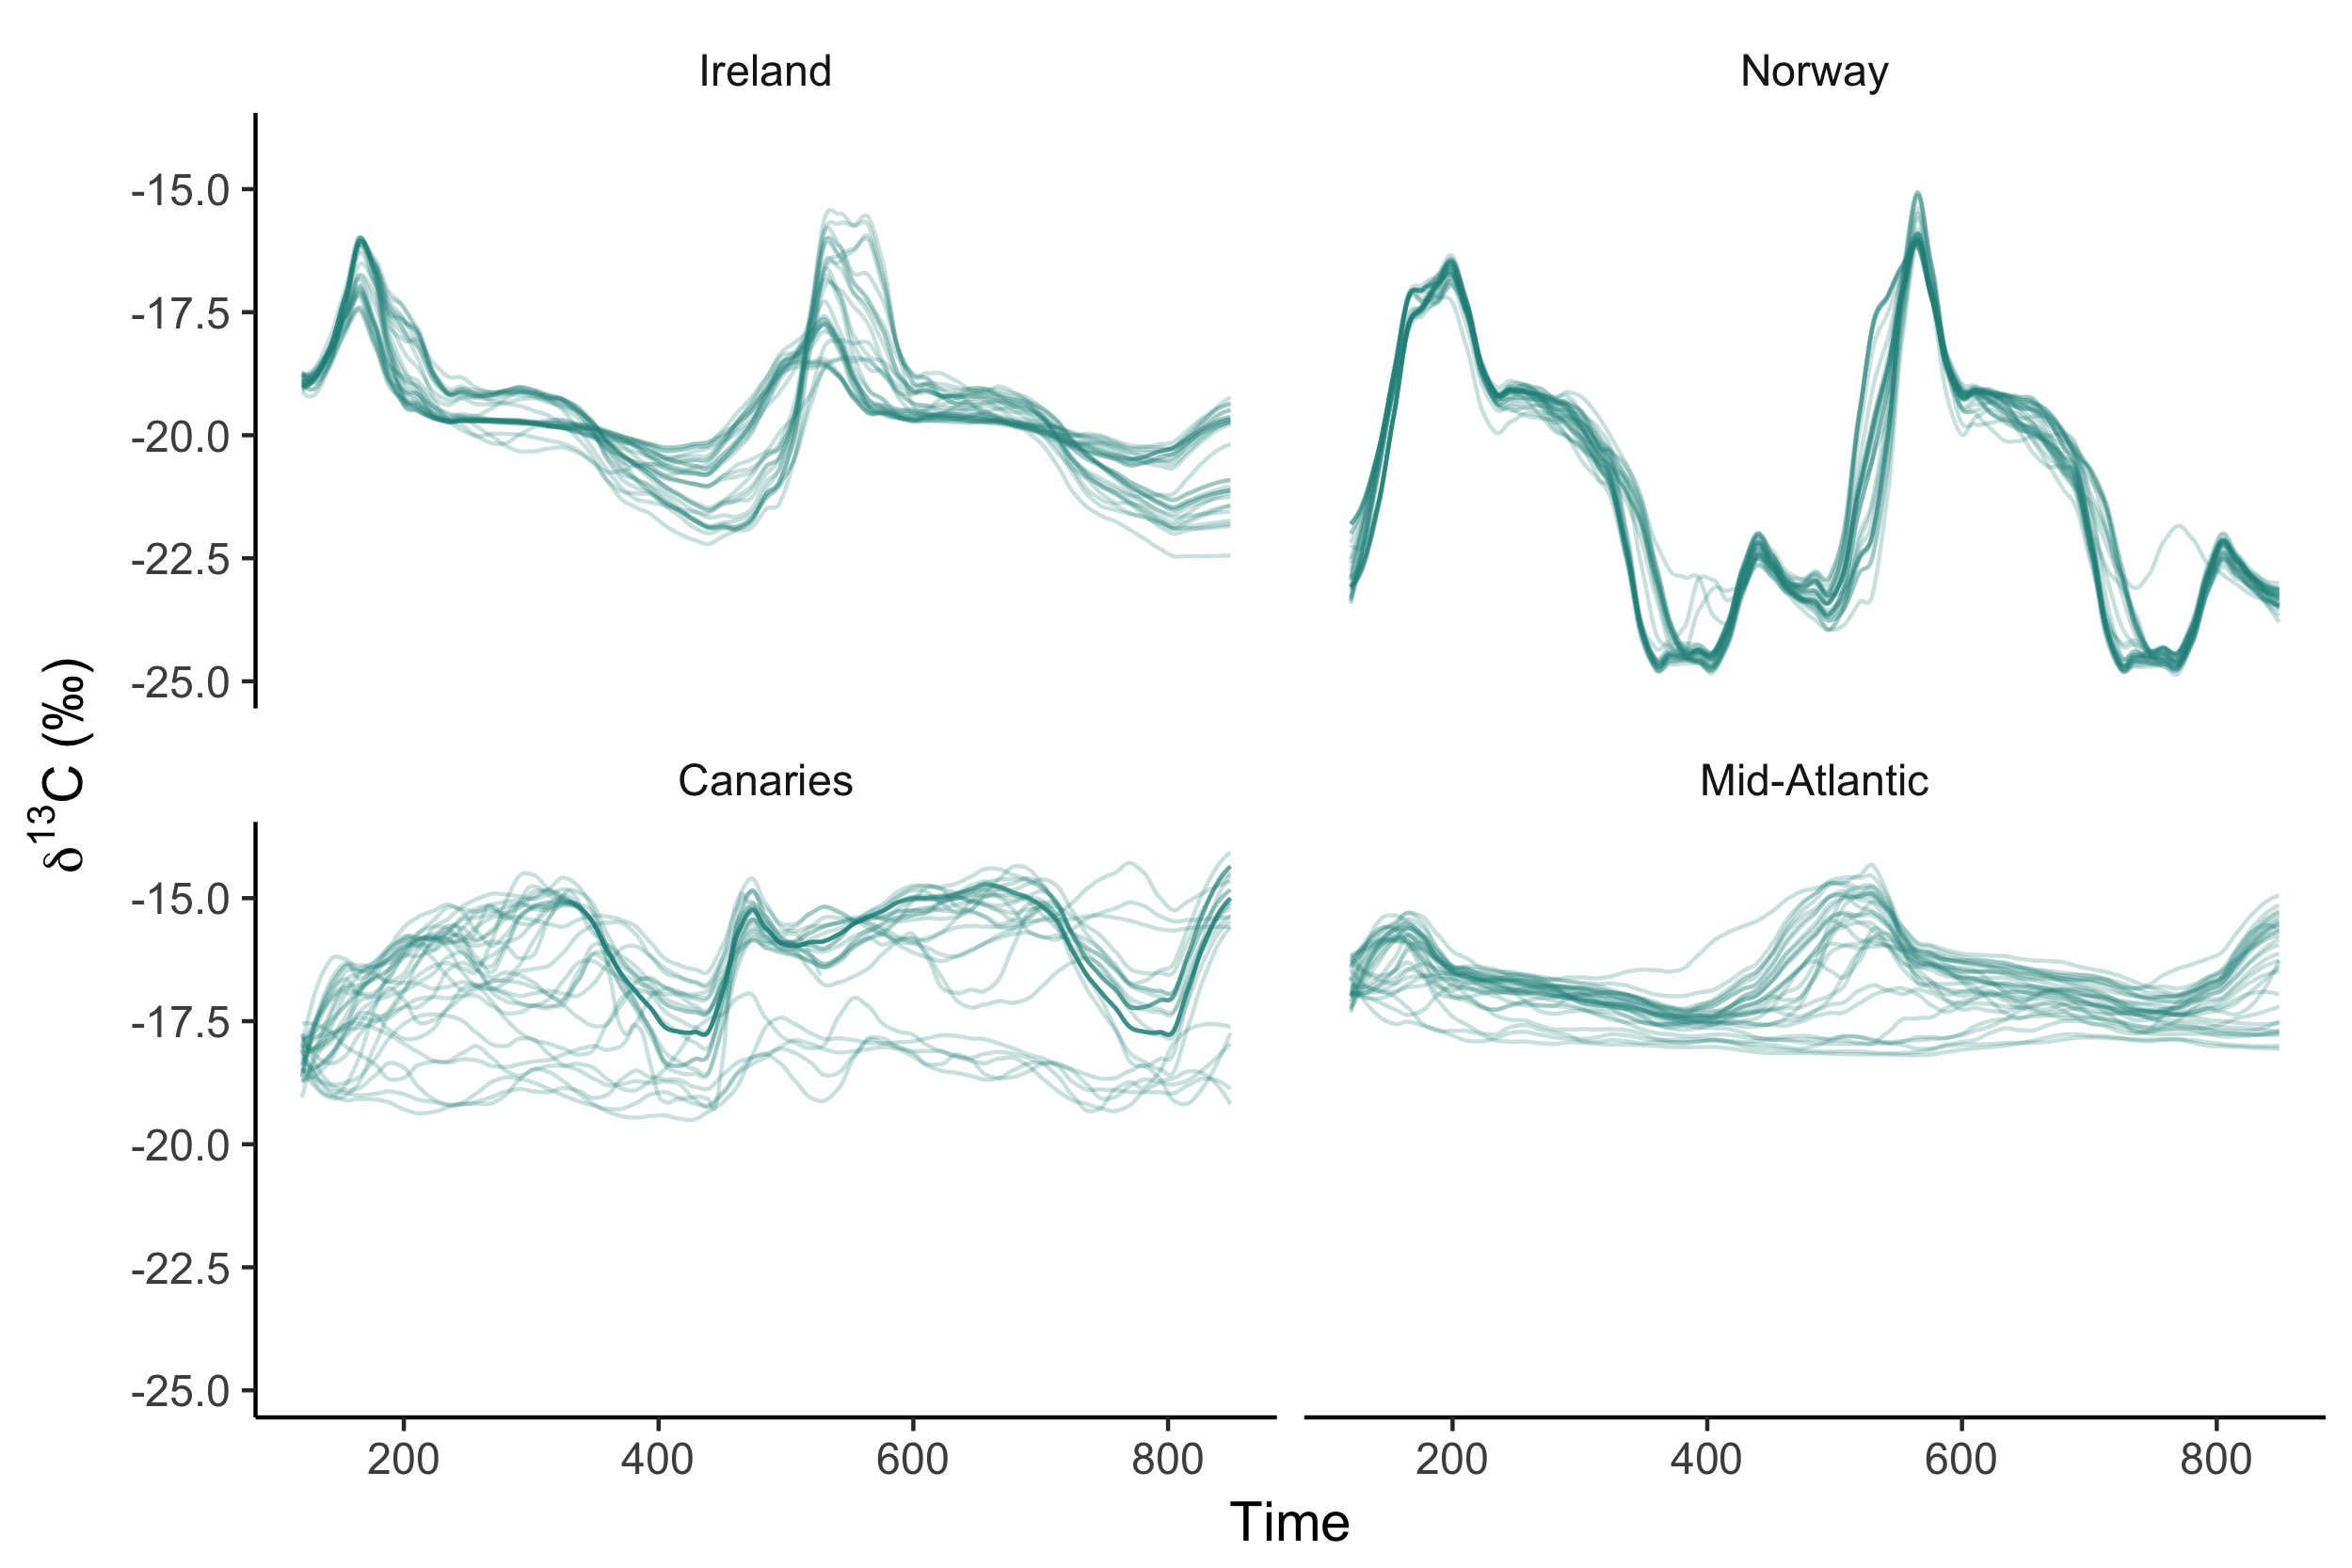
\includegraphics[width=\linewidth]{figures/Figure-S4-facet-wrap-d13C.png}
      \caption{Alternative $\delta^{13}$C series arising from resident-only movement models restricting region to west UK/Irish shelf (Ireland), Norwegian/Barents Sea (Norway), Canaries/west Azores (Canaries), Mid Atlantic ridge (Mid-Atlantic), over a simulated two year period with daily resolution and 30 replicate simulations for each region.} % check legend
      \label{figs4}
  \end{figure}
 
\subsubsection*{Matching isotope model simulations with whale isotopes in behavioural phase one}
Behavioural phase one is characterised by approximately 24 months of relatively positive and constant $\delta^{13}$C values. 
$\delta^{15}$N values in this phase are relatively low and the isotopic cyclicity is absent (Fig. \ref{figs1}). 
Positive and temporally constant $\delta^{13}$C values are characteristic of subtropical regions particularly upwelling areas around Mauritania, Cape Verde and the Azores region.
 
\subsubsection*{Matching isotope model simulations with whale isotopes in behavioural phase two}
Temporal dynamics in $\delta^{13}$C values simulated in northerly latitudes cannot be reproduced from simulated temporal trends in $\delta^{13}$C values in krill within static areas (Fig. \ref{figs4}, Fig. 3). 
Adding seasonal north-south migrations within mid-high latitude regions to foraging models, closely matches the measured profile, including $\delta^{13}$C minima preceding the June bloom (Fig. \ref{figs4}, Fig. 1).

Accordingly we modeled whale movements allowing three years of residency in warm waters of the Azores or Cape Verde/Mauritania region followed by a further 3.5 years of seasonal north-south migration in the northeast northern Atlantic, followed by residency in subtropical waters in 1890 and rapid migration returning to more northerly waters in the spring of 1891. 
The resulting simulated profiles closely match the measured baleen plate, capturing all major temporal fluctuations (Fig. 3). 
Blue whales have a gestation period of 10-12 months, and calves suckle for approximately 6-7 months \cite{handbook}. 
The proposed timescale of pregnancy around early spring 1889, birth in spring 1890, lactation through summer and autumn 1890 and return to northern feeding grounds in early 1891 is therefore fully consistent with the assumed reproductive ecology of blue whales.

\subsection*{AGENT-BASED WHALE MOVEMENT MODEL}
We simulated the likely isotopic expression associated with feeding and movement behaviours by building an agent-based model sampling $\delta^{13}$C POM values predicted by the isotopic extension to the NEMO-MEDUSA model\cite{magozzi2017using,yool2013medusa}, where movement behavior is influenced by sea surface temperature and phytoplankton biomass estimates provided by NEMO-MEDUSA\cite{yool2013medusa}, and bathymetry (Fig. \ref{figs5}).
 
The agent-based model developed employs a simple set of movement rules dictated by behavioural state which is itself fixed according to calendar month by the operator. 
At each daily step, the probability of movement, movement direction and distance traveled are sampled from probability distributions to allow individual variation.

Initial boundary conditions are defined with a maximum temperature of 25$^{\circ}$C and minimum temperature of 3$^{\circ}$C. The likelihood of movement (i.e. whether to move or not from the current location) is sampled from a binomial distribution with the probability of movement influenced by behavioural state and external conditions. 
The maximum daily movement distance permitted in each behavioural state is defined as a random sample of a Gaussian distribution with specified mean and standard deviation (see Table \ref{tables1}).
 
The behavioural states employed in the model simulations are foraging, migrating north and migrating south. When foraging, the probability of movement and likely direction of movement is primarily controlled by the biomass of phytoplankton in the current and adjacent 1$^{\circ}$ cells. When migrating, a fixed higher probability of movement is given to southerly or northerly movement directions, and the probability of movement is influenced by the ambient sea surface temperature and phytoplankton biomass.
 
Parameters defined for the agent-based model best matching the measured profile are summarised in Table \ref{tables1}.

\newpage

\begin{landscape}

  \vspace{-1cm}
\begin{figure}[!htbp]
  \centering
  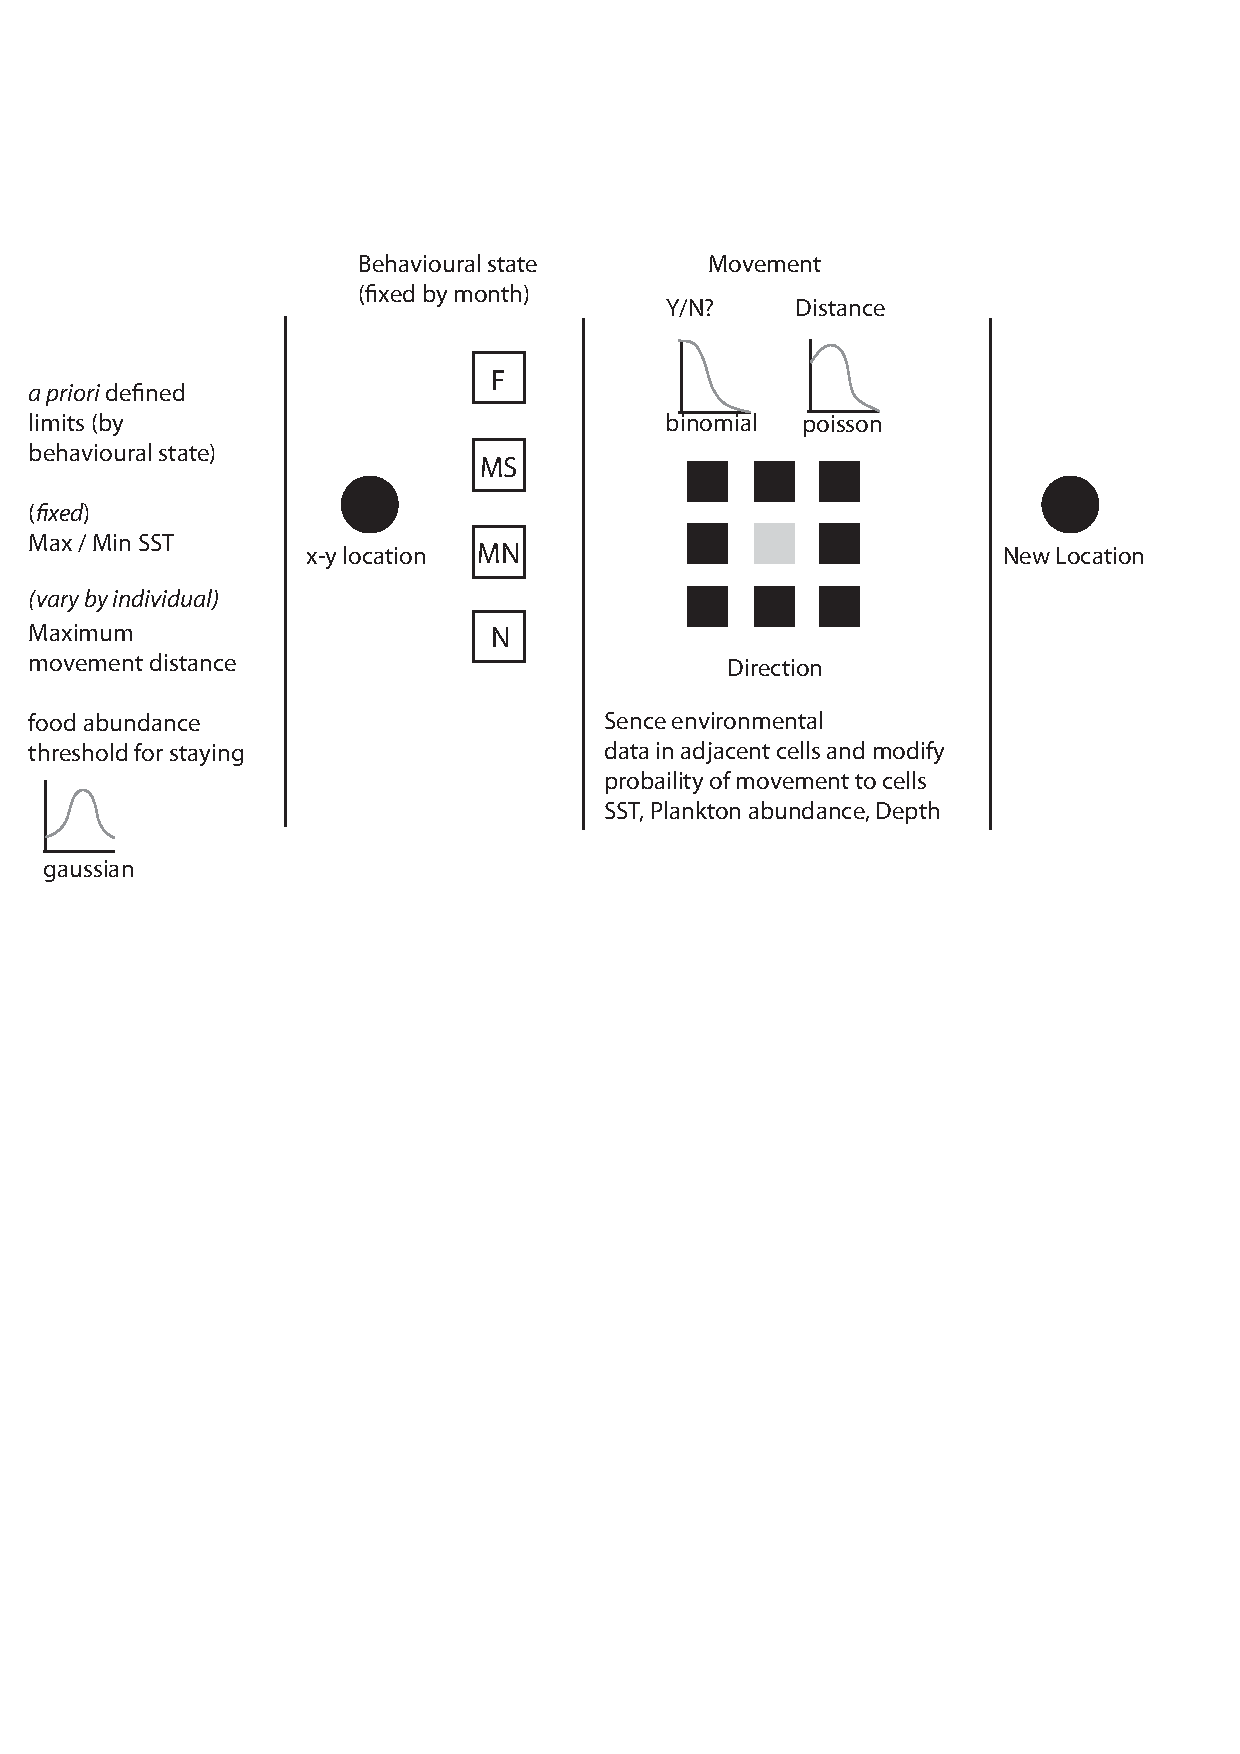
\includegraphics[trim = 0cm 145mm 0cm 4cm, clip]{figures/flow-diagram-model.pdf}
  \vspace{-1.2cm}
  \linespread{0.8}
  \caption{
  Schematic structure of the agent-based model used to generate hypothetical movement tracks. 
  At the start of each simulation, max and min sea surface temperature (SST) and food availability thresholds are fixed for all individuals. Behavioural states are defined \textit{a priori} based on day of the year. Maximum movement distances under each behavioural state are defined for each individual based on a random sample from a Gaussian distribution. The model runs with a daily time step. Current location and day of simulation is noted, and the behavioural state defined. Environmental conditions (SST, food availability and depth) are sensed in the current and eight adjacent 1$^{\circ}$ grid cells. The probability of movement is sampled from a binomial distribution defined according to behavioural state and environmental conditions in the current location. The direction of movement is sampled based on discrete probabilities associated to each of the eight adjacent 1$^{\circ}$ cells, defined according to behavioural state and environmental conditions. Finally the distance moved is sampled from a Poisson distribution conditional on the maximum distance defined for each individual. The new location is then assigned from a linear vector originating at the current location with magnitude defined as the distance moved and direction as 45$^{\circ}$ increments reflecting the relative orientation of each of the eight potential adjacent cells.}
  \label{figs5}
\end{figure}

\newpage

\centering
\begin{table}
  \begin{tabular}{|p{8cm}|c|c|c|} 
    \hline
    & \multicolumn{3}{|c|}{\textbf{Behavioural state}} \\
    \hline
    \textbf{Parameters} & \textbf{Foraging} & \textbf{Migrating north} & \textbf{Migrating south}\\
    \hline
    Behavioural phase one (1095 days) & Jan - Dec & NA & NA\\
    \hline
    Behavioural phase two (1278 days) & June - Oct & April - May & Nov - March\\
    \hline
    Pregnancy, nursing, return (447 days) & Jan - Dec & NA & NA\\
    \hline
    Post nursing migration (100 days) & NA & Jan - June & NA\\
    \hline
    Minimum sea surface temperature$^*$ ($^{\circ}$C) & 3 & 3 & 3\\
    \hline
    Maximum sea surface temperature ($^{\circ}$C) & 25 & 25 & 25\\
    \hline
    Maximum daily distance traveled (km)$^{**}$ & $N(\mu=50, \sigma=25)$ & $N(\mu=150, \sigma=75)$ & $N(\mu=150, \sigma=75)$\\
    \hline
    Plankton biomass threshold for remaining to forage (units) & 50 & NA & NA\\
    \hline
  \end{tabular}
  \caption{Model parameters for agent-based model of whale movement. 
  See Fig. \ref{figs5} and text for more details. 
  $^*$During nursing minimum sea surface temperature is set to 18$^{\circ}$C. 
  $^{**}$During behavioural phase one, mean maximum daily distance is set to 20km.}
  \label{tables1}
\end{table}

\end{landscape}

\newpage

\subsection*{ADDITIONAL RESULTS FIGURES}

  \begin{figure}[!htbp]
    \centering
      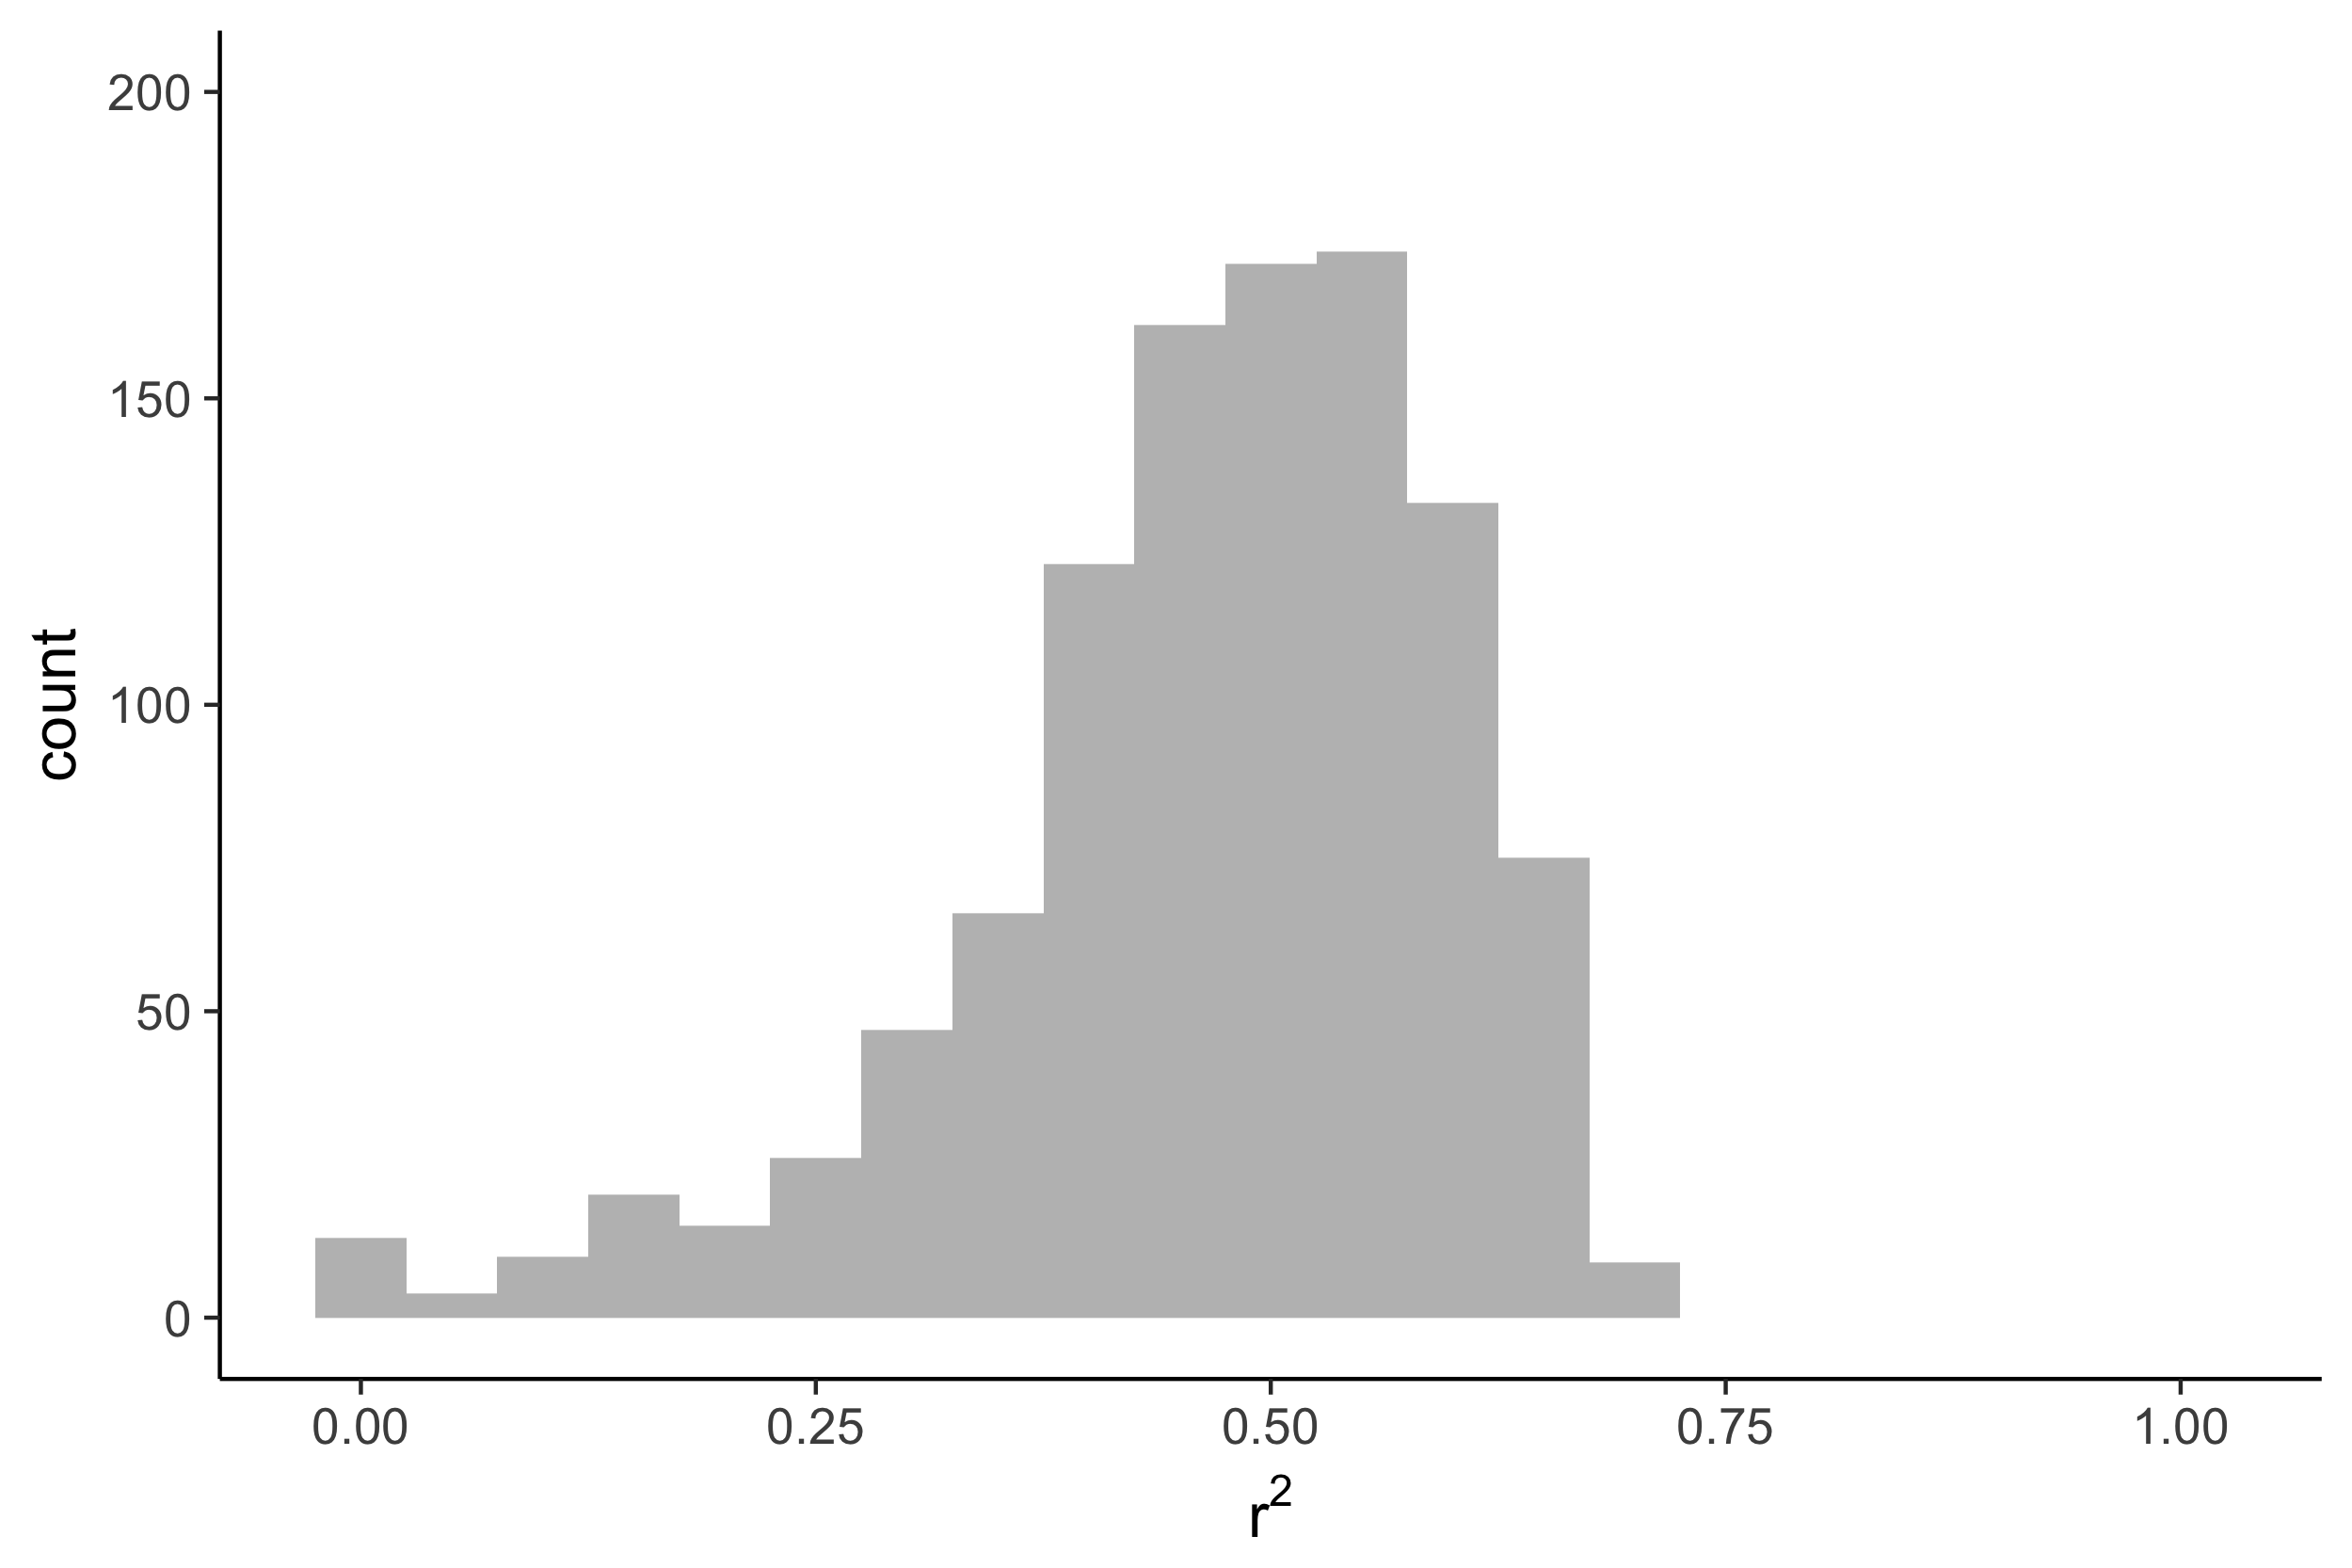
\includegraphics[width=\linewidth]{figures/Figure-S5-r2.png}
      \caption{Histogram of $r^2$ values from linear regressions comparing model simulation $\delta^{13}$C values to those of the real data (Fig. 1).} % check legend
      \label{figs6}
  \end{figure}

    \begin{figure}[!htbp]
    \centering
      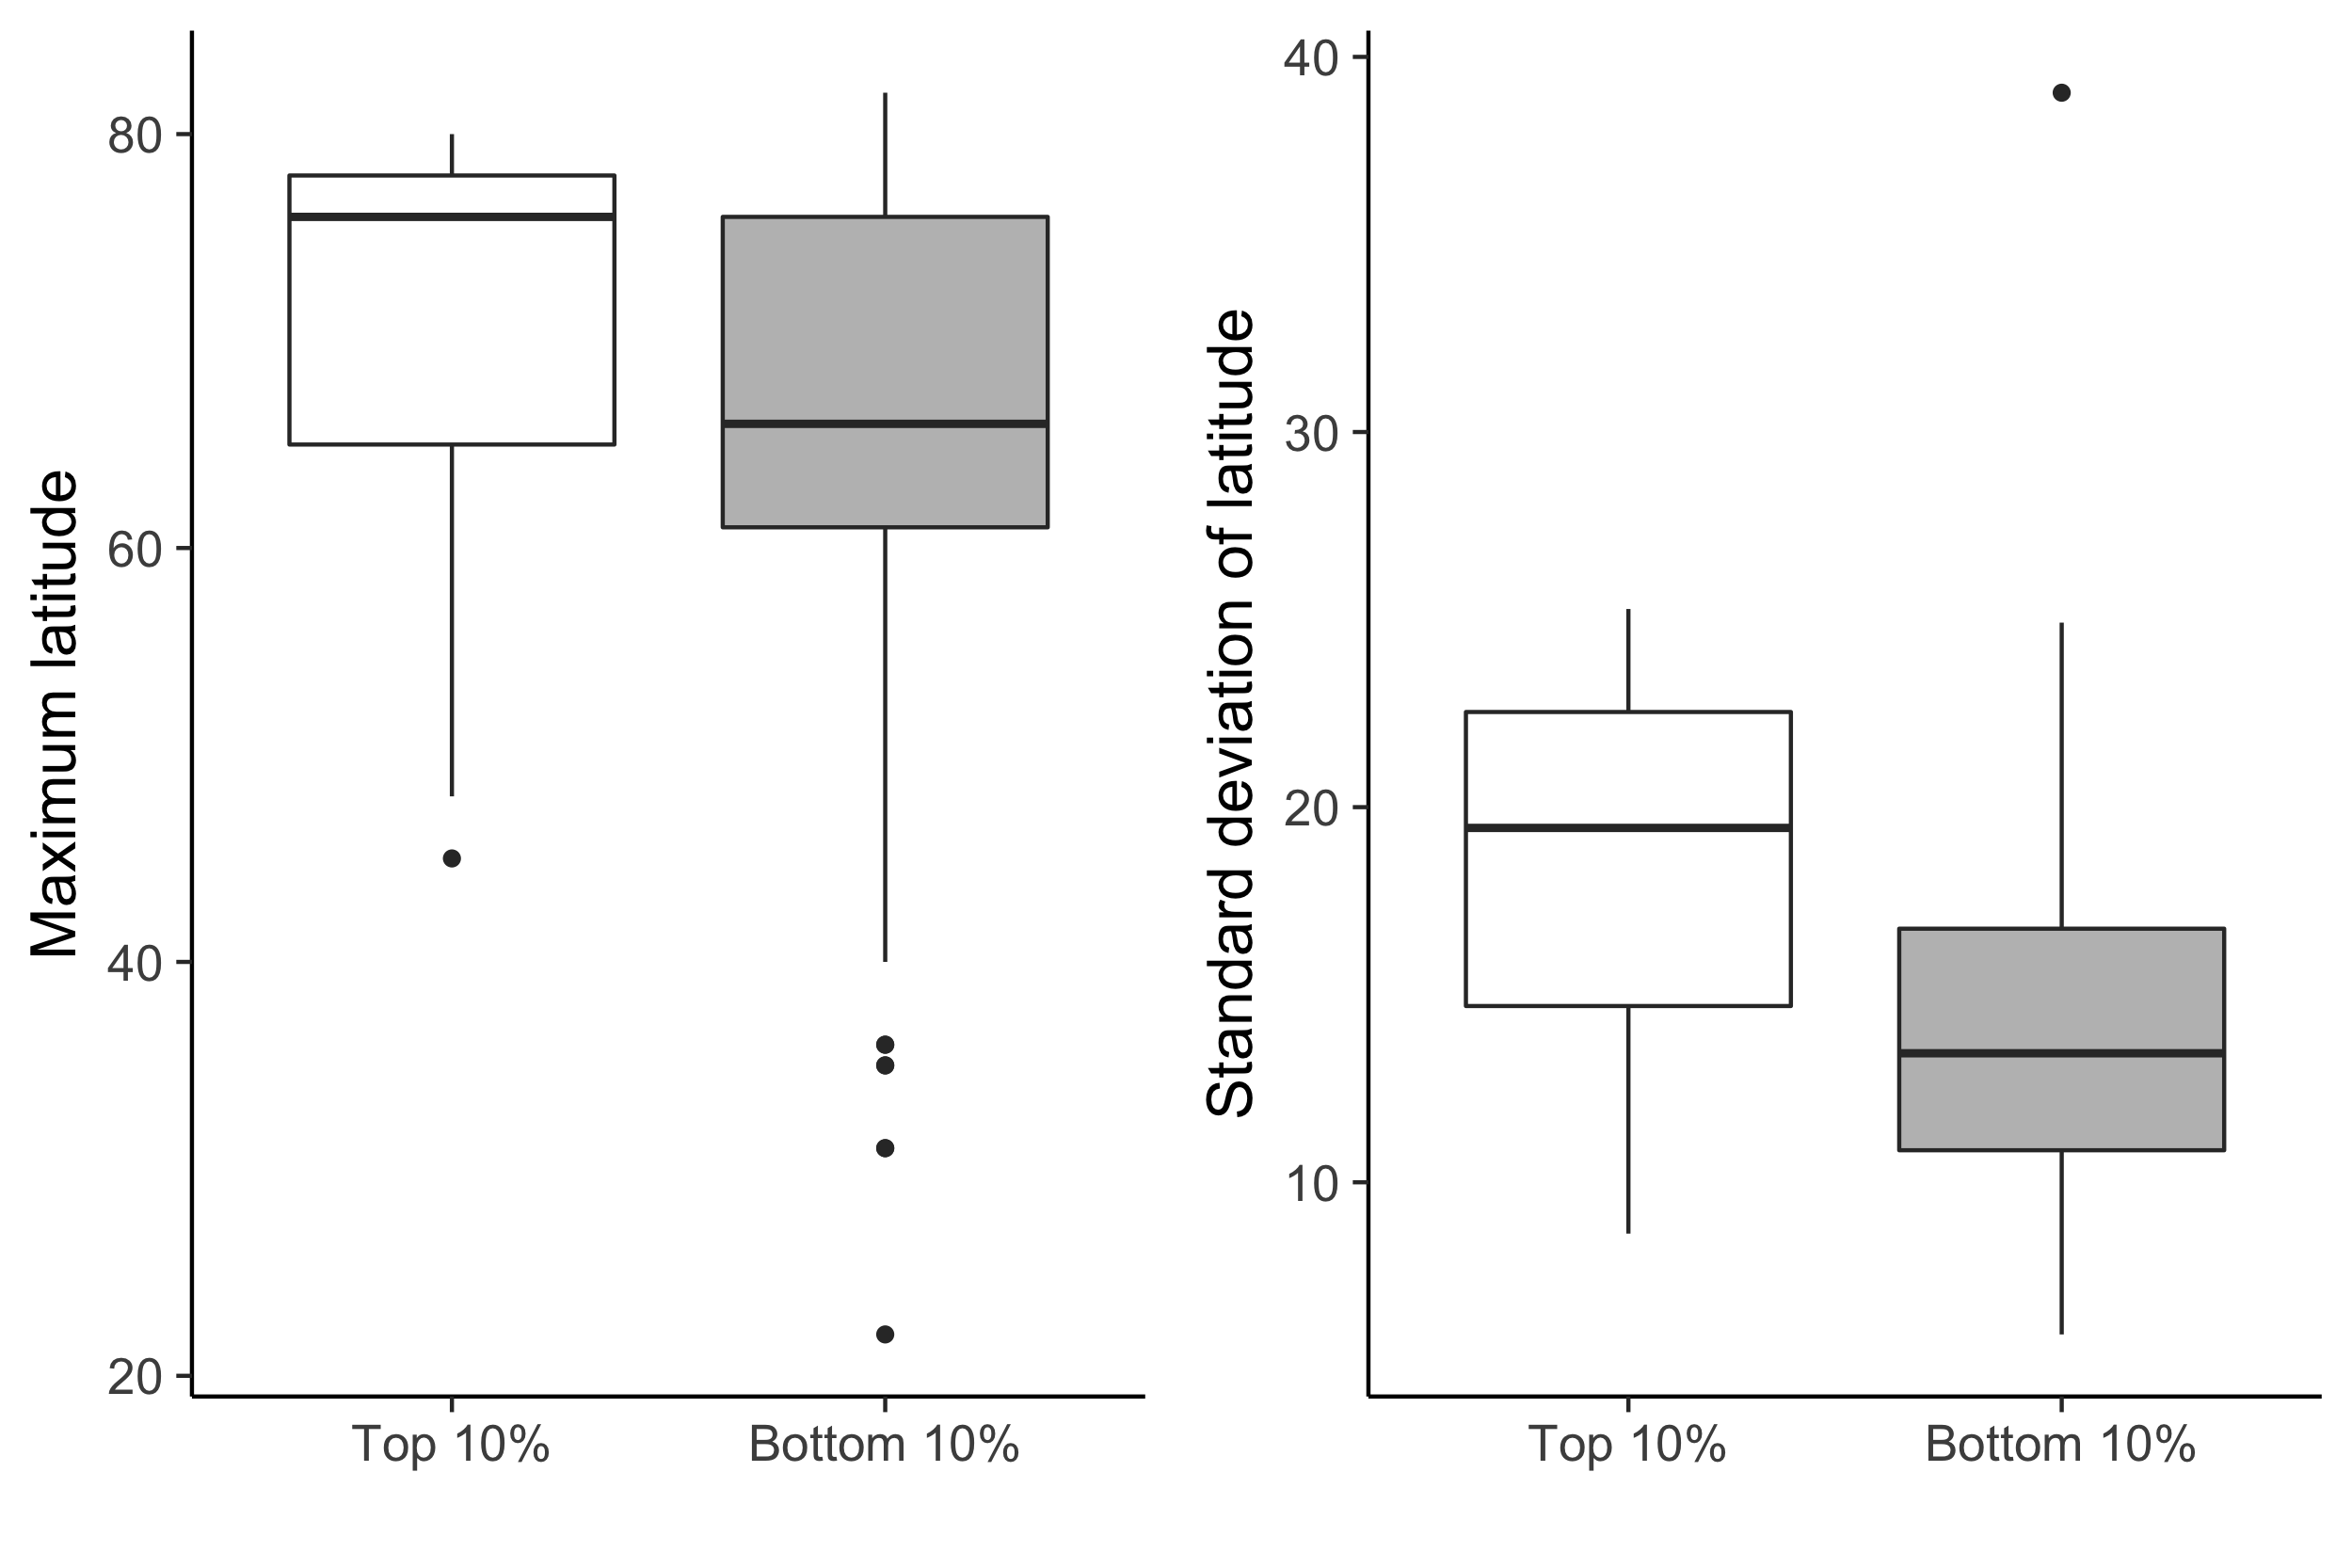
\includegraphics[width=\linewidth]{figures/Figure-S6-boxplots.png}
      \caption{Boxplots showing the maximum and standard devations of latitudinal positions of simulated whales taken from the top 10\%, and bottom 10\%, of movement model simulations.} % check legend
      \label{figs7}
  \end{figure}

    \begin{figure}[!htbp]
    \centering
      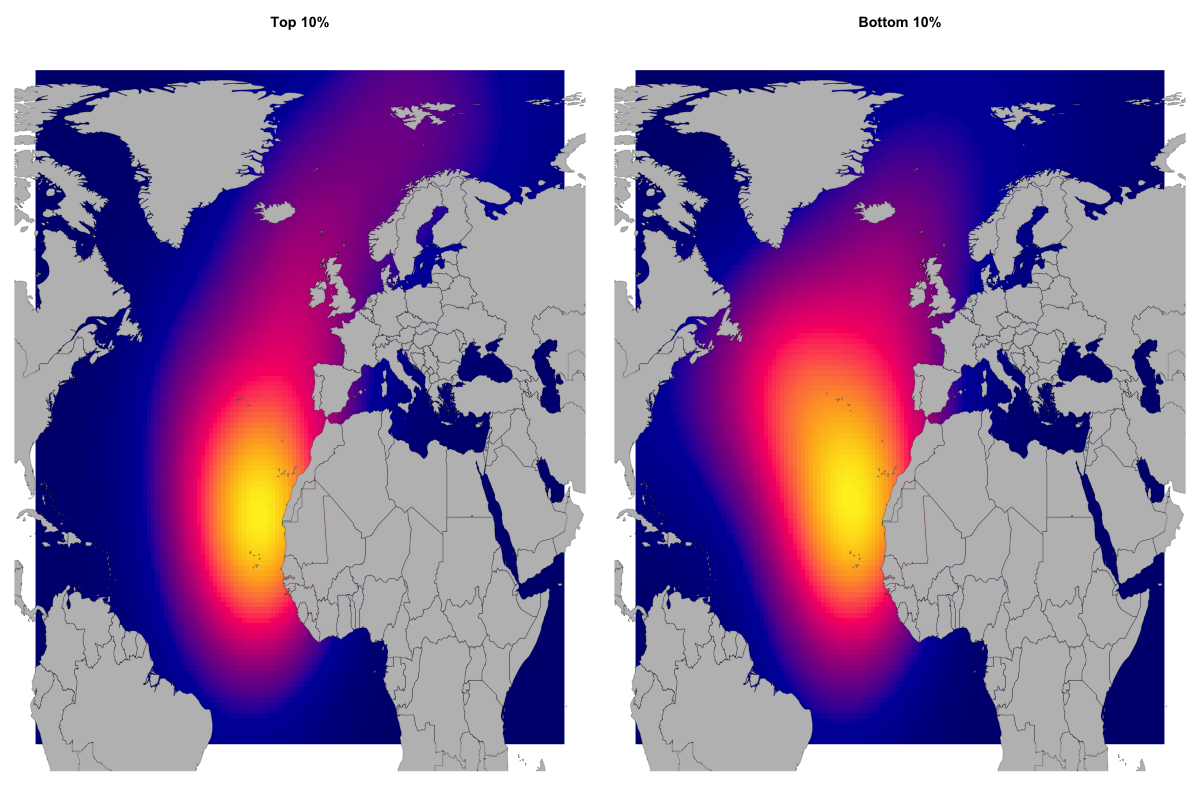
\includegraphics[width=\linewidth]{figures/Figure-S7-kernals.png}
      \caption{Kernal density plots showing the positions of simulated whales taken from the top 10\%, and bottom 10\%, of movement model simulations. 
      High densities are in yellow, low densities are in blue.} % check legend
      \label{figs8}
  \end{figure}
 
% References
\newpage
\bibliographystyle{nature}
\bibliography{blue-whale}

\end{document}